%%%%%%%%%%%%%%%%%%%%%%%%%%%%%%%%%%%%%%%%%%%%%%%%%%%%%%%%%%%%%%%%%%%%%%%%%%%%
% 26/05/2010
% edited by Bill Lampos
%
% Feel free to use (copy) the structure (latex formatting source code)
% but not the content of this document.
%
%%%%%%%%%%%%%%%%%%%%%%%%%%%%%%%%%%%%%%%%%%%%%%%%%%%%%%%%%%%%%%%%%%%%%%%%%%%%%
\documentclass[mathserif,compress,red]{beamer}
\mode<presentation>

\usetheme{Warsaw}
% other themes: AnnArbor, Antibes, Bergen, Berkeley, Berlin, Boadilla, boxes, CambridgeUS, Copenhagen, Darmstadt, default, Dresden, Frankfurt, Goettingen,
% Hannover, Ilmenau, JuanLesPins, Luebeck, Madrid, Maloe, Marburg, Montpellier, PaloAlto, Pittsburg, Rochester, Singapore, Szeged, classic

\usecolortheme{default}
% color themes: albatross, beaver, beetle, crane, default, dolphin, dov, fly, lily, orchid, rose, seagull, seahorse, sidebartab, structure, whale, wolverine

%\usefonttheme{serif}
% font themes: default, professionalfonts, serif, structurebold, structureitalicserif, structuresmallcapsserif

% pdf is displayed in full screen mode automatically
%\hypersetup{pdfpagemode=FullScreen}

% define your own colours:
\definecolor{Red}{rgb}{1,0,0}
\definecolor{Blue}{rgb}{0,0,1}
\definecolor{Green}{rgb}{0,1,0}
\definecolor{magenta}{rgb}{1,0,.6}
\definecolor{lightblue}{rgb}{0,.5,1}
\definecolor{lightpurple}{rgb}{.6,.4,1}
\definecolor{gold}{rgb}{.6,.5,0}
\definecolor{orange}{rgb}{1,0.4,0}
\definecolor{hotpink}{rgb}{1,0,0.5}
\definecolor{newcolor2}{rgb}{.5,.3,.5}
\definecolor{newcolor}{rgb}{0,.3,1}
\definecolor{newcolor3}{rgb}{1,0,.35}
\definecolor{darkgreen1}{rgb}{0, .35, 0}
\definecolor{darkgreen}{rgb}{0, .6, 0}
\definecolor{darkred}{rgb}{.75,0,0}

\xdefinecolor{olive}{cmyk}{0.64,0,0.95,0.4}
\xdefinecolor{purpleish}{cmyk}{0.75,0.75,0,0}

% \usepackage{beamerinnertheme_______}
% inner themes include circles, default, inmargin, rectangles, rounded

%\usepackage{beamerouterthemesmoothbars}
% outer themes include default, infolines, miniframes, shadow, sidebar, smoothbars, smoothtree, split, tree

\useoutertheme[subsection=false]{smoothbars}

% to have the same footer on all slides
%\setbeamertemplate{footline}[text line]{xxx xxx xxx}
%\setbeamertemplate{footline}[text line]{} % or empty footer

% include packages
\usepackage{etex}
\usepackage{subfigure}
\usepackage{multicol}
\usepackage{amsmath}
\usepackage{epsfig}
\usepackage{graphicx}
\usepackage[all,knot]{xy}
\xyoption{arc}
\usepackage{url}
\usepackage{multimedia}
\usepackage{hyperref}
\usepackage{setspace}
\usepackage{verbatim}
\usepackage{enumerate}

\title{MTiG Position Sensor Accuracy Test}
\author{John Liu}
\institute{{\tiny Advisor:}\\ \vspace{.10cm}Professor Ying-Jeng Wu}
\date{\scriptsize Measurement Laboratory, National Yunlin University of Science \& Technology\\ \vspace{.10cm}April 24, 2014}

\begin{document}

\frame{
	\titlepage
}

\section{Outline}
\frame{\tableofcontents}

\section{Stationary Test}
\frame{\frametitle{Stationary Test: Test 1}
$\sigma = 2.967$

Average Satellite Number $N = 8.14$
\begin{figure}[h!]
	\centering
	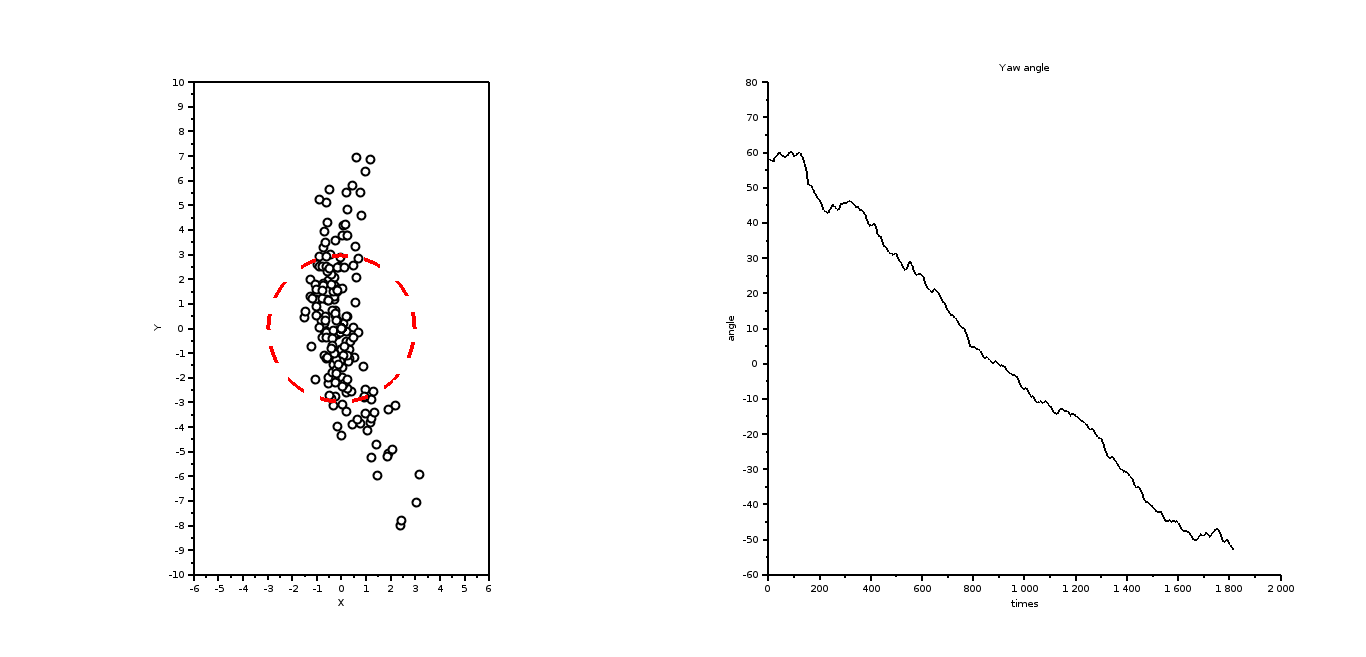
\includegraphics[scale=.23]{figures/stationary_test_1.png}
\end{figure}
}

\frame{\frametitle{Stationary Test: Test 2}
$\sigma = 1.819$

$N = 7.92$
\begin{figure}[h!]
	\centering
	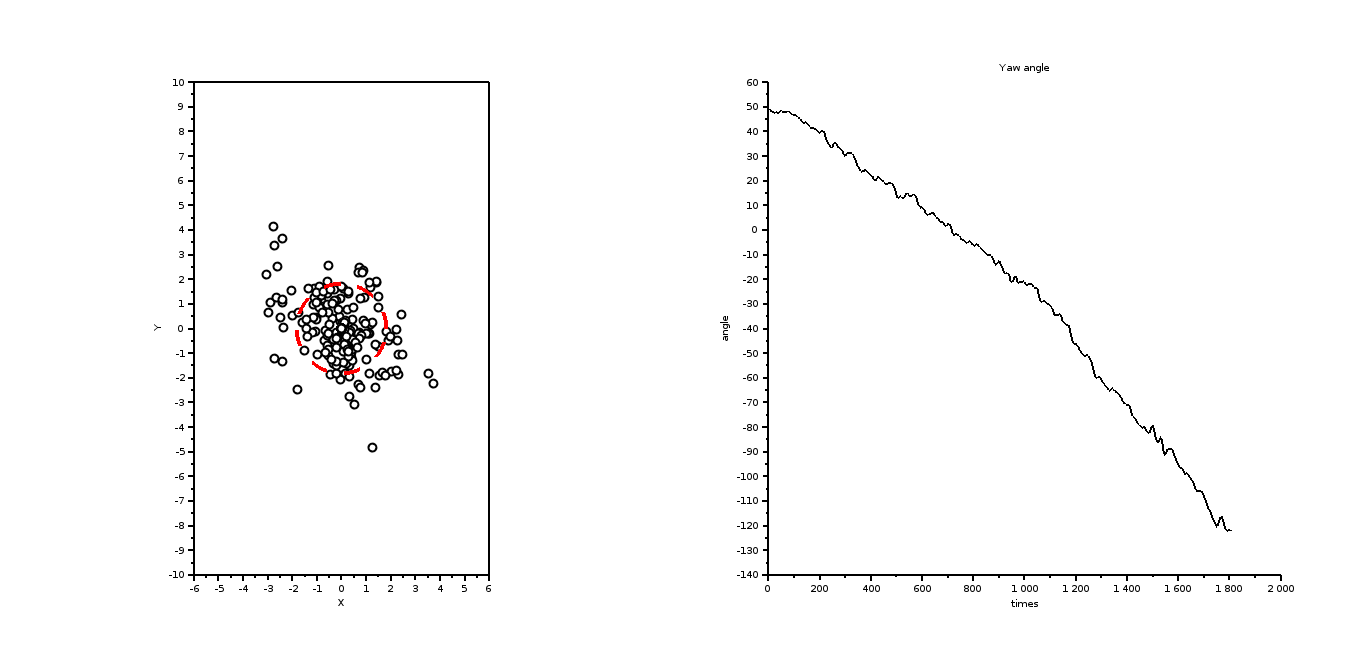
\includegraphics[scale=.23]{figures/stationary_test_2.png}
\end{figure}
}

\section{Dynamic Test}
\frame{\frametitle{Dynamic Test: Test 1}
\begin{columns}
	\begin{column}{5cm}
		\centering
		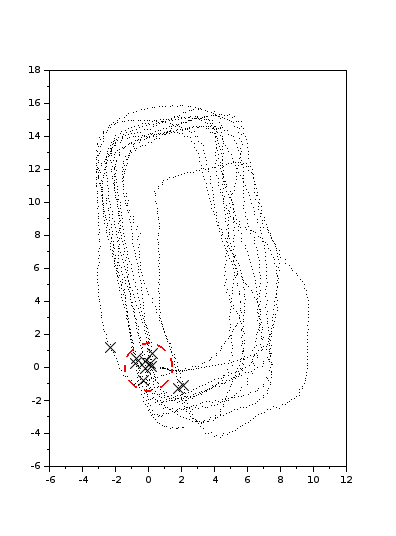
\includegraphics[scale=.41]{figures/dynamic_1.png}
	\end{column}
	\begin{column}{5cm}
		Date: 2014/04/22

		Time: 10:30

		$\sigma = 1.435$

		$N = 6.81$
	\end{column}
\end{columns}
}

\frame{\frametitle{Dynamic Test: Test 2}
\begin{columns}
	\begin{column}{5cm}
		\centering
		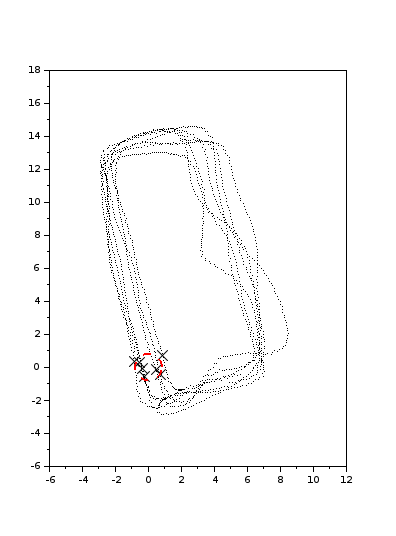
\includegraphics[scale=.41]{figures/dynamic_2.png}
	\end{column}
	\begin{column}{5cm}
		Date: 2014/04/22

		Time: 15:30

		$\sigma = 0.807$

		$N = 8.24$
	\end{column}
\end{columns}
}

\frame{\frametitle{Dynamic Test: Test 3}
\begin{columns}
	\begin{column}{5cm}
		\centering
		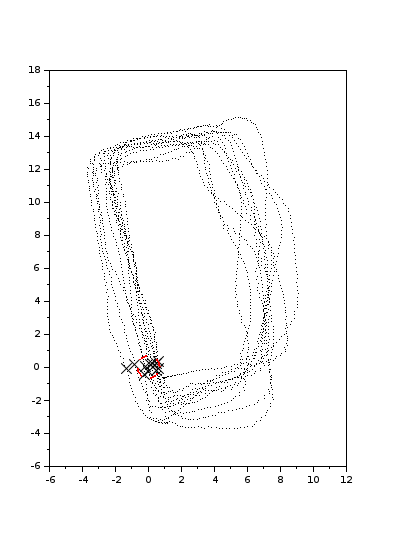
\includegraphics[scale=.41]{figures/dynamic_3.png}
	\end{column}
	\begin{column}{5cm}
		Date: 2014/04/22

		Time: 20:30

		$\sigma = 0.668$

		$N = 7.95$
	\end{column}
\end{columns}
}

\frame{\frametitle{Dynamic Test: Test 4}
\begin{columns}
	\begin{column}{5cm}
		\centering
		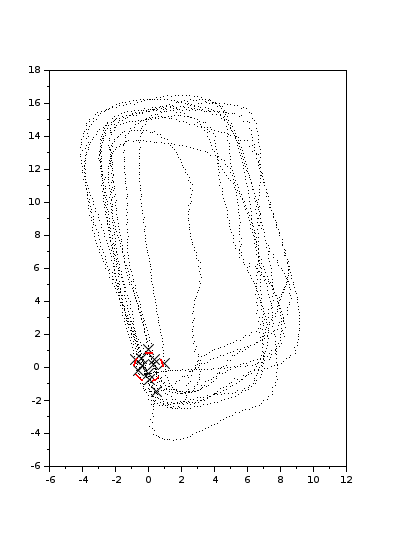
\includegraphics[scale=.41]{figures/dynamic_4.png}
	\end{column}
	\begin{column}{5cm}
		Date: 2014/04/23

		Time: 10:30

		$\sigma = 0.871$

		$N = 5.92$
	\end{column}
\end{columns}
}

\frame{\frametitle{Dynamic Test: Test 5}
\begin{columns}
	\begin{column}{5cm}
		\centering
		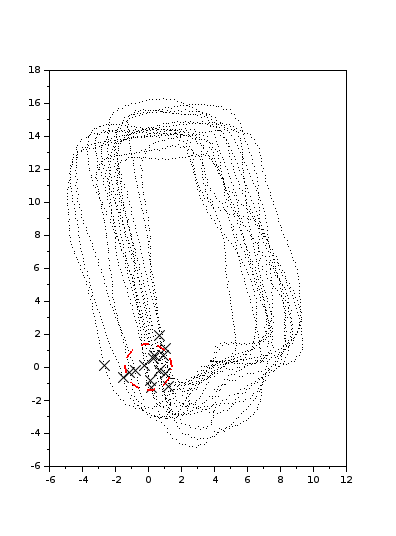
\includegraphics[scale=.41]{figures/dynamic_5.png}
	\end{column}
	\begin{column}{5cm}
		Date: 2014/04/23

		Time: 15:30

		$\sigma = 1.400$

		$N = 5.76$
	\end{column}
\end{columns}
}

\frame{\frametitle{Dynamic Test: Test 6}
\begin{columns}
	\begin{column}{5cm}
		\centering
		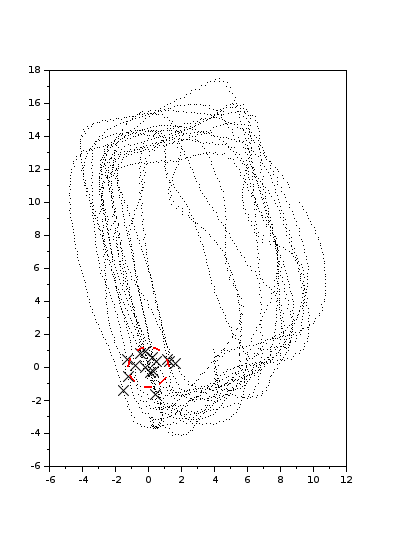
\includegraphics[scale=.41]{figures/dynamic_6.png}
	\end{column}
	\begin{column}{5cm}
		Date: 2014/04/23

		Time: 20:30

		$\sigma = 1.217$

		$N = 7.90$
	\end{column}
\end{columns}
}

\frame{\frametitle{Dynamic Test: Test 7}
\begin{columns}
	\begin{column}{5cm}
		\centering
		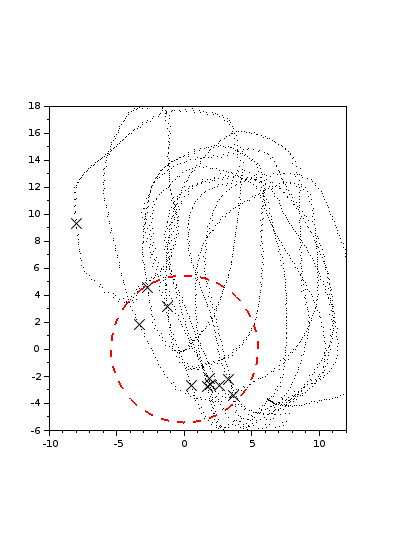
\includegraphics[scale=.41]{figures/dynamic_7.png}
	\end{column}
	\begin{column}{5cm}
		Date: 2014/04/24

		Time: 10:30

		$\sigma = 5.446$

		$N = 5.47$
	\end{column}
\end{columns}
}

\frame{\frametitle{Dynamic Test: Test 8}
\begin{columns}
	\begin{column}{5cm}
		\centering
		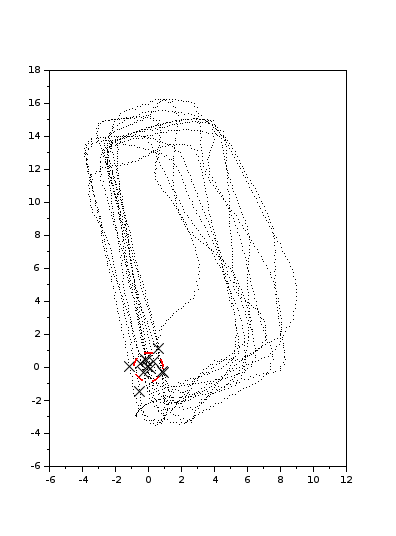
\includegraphics[scale=.41]{figures/dynamic_8.png}
	\end{column}
	\begin{column}{5cm}
		Date: 2014/04/24

		Time: 15:30

		$\sigma = 0.876$

		$N = 5.89$
	\end{column}
\end{columns}
}

\frame{\frametitle{Dynamic Test: Test 9}
\begin{columns}
	\begin{column}{5cm}
		\centering
		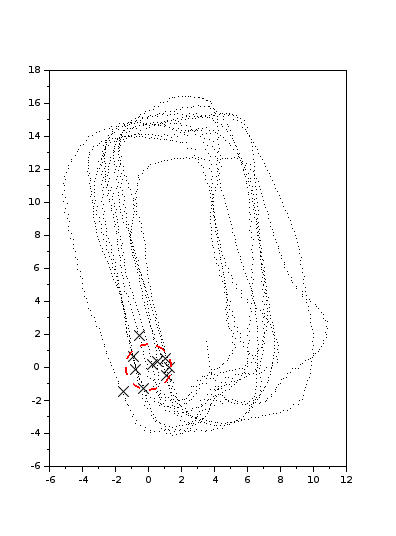
\includegraphics[scale=.41]{figures/dynamic_9.png}
	\end{column}
	\begin{column}{5cm}
		Date: 2014/04/24

		Time: 20:30

		$\sigma = 1.375$

		$N = 7.00$ 
	\end{column}
\end{columns}
}

\frame{\frametitle{Dyanmic Test: Time Dependence}
\begin{figure}
	\centering
	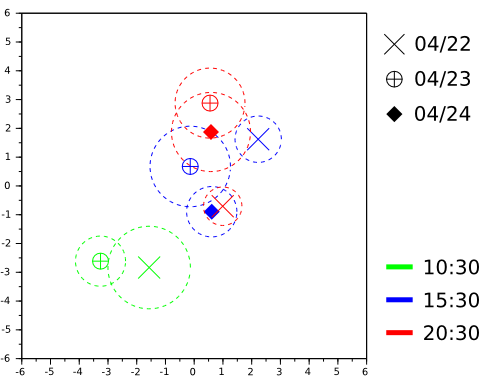
\includegraphics[scale=.60]{figures/timediff.png}
\end{figure}
}

\frame{\frametitle{Dyanmic Test: Satellite Number Dependence}
\begin{figure}
	\centering
	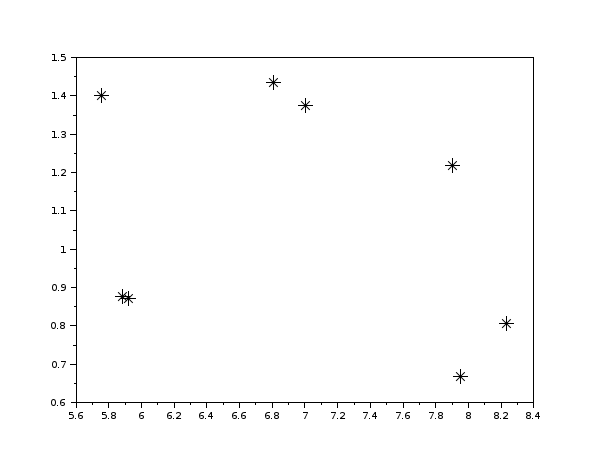
\includegraphics[scale=.45]{figures/Sigma-N.png}
\end{figure}
}

\section{Conclusion}

\frame{\frametitle{Conclusion}
\begin{enumerate}
	\vspace{0.25cm}
	\item Measurement of yaw angle cannot converged without movement.
	\vspace{0.25cm}
	\item Measurement of position depends on measuring time.
	\vspace{0.25cm}
	\item The is no correlation between accuracy and satellite number. 
\end{enumerate}
}


\begin{comment}
\section{Common Obstacle Avoidance Overview}
\subsection{Artificial Potential Field}
\frame{\frametitle{Artificial Potential Field}
Artificial Potential Field creates a virtual force field which attracts the robot toward the target, and retracts it away from the obstacle.
\begin{columns}
	\begin{column}{5cm}
	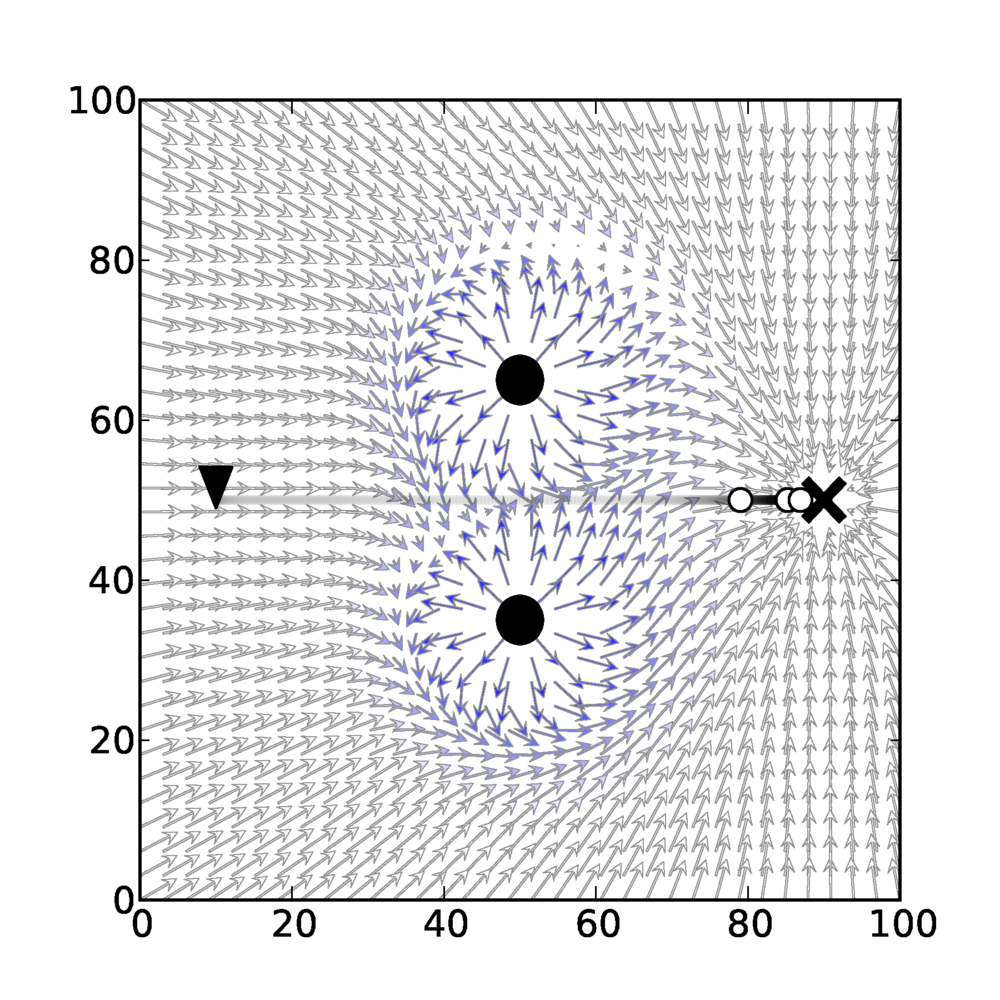
\includegraphics[scale=.18]{figures/APF.png}
	\end{column}
	\begin{column}{5cm}
	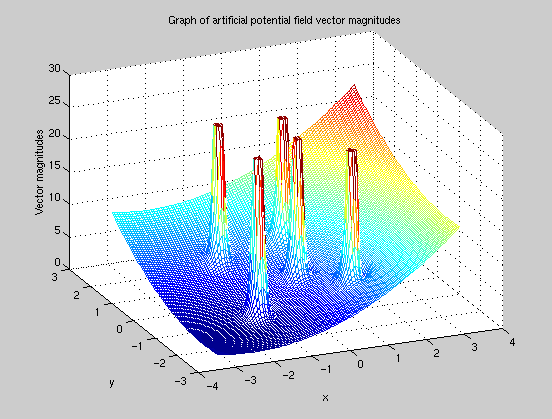
\includegraphics[scale=.25]{figures/demo_apf.png}
	\end{column}
\end{columns}
}

\frame{\frametitle{Artificial Potential Field}
\begin{itemize}
	\item Advantages:
	\begin{itemize}
		\item Global path planning
		\item Efficient Calculation
		\item Easily adapt to the data acquired by LiDAR
	\end{itemize}
	\vspace{0.25cm}
	\item Disadvantages:
	\begin{itemize}
		\item Ignore the kinematic and dynamic constraints
		\item Ignore robot's geometry
	\end{itemize}
\end{itemize}
}

\subsection{Vector Field Histogram}
\frame{\frametitle{Vector Field Histogram (VFH)}
VFH generates a polar histogram of the environment around the robot, identifies wide-enough spaces and calculates corresponding steering direction.
\begin{figure}
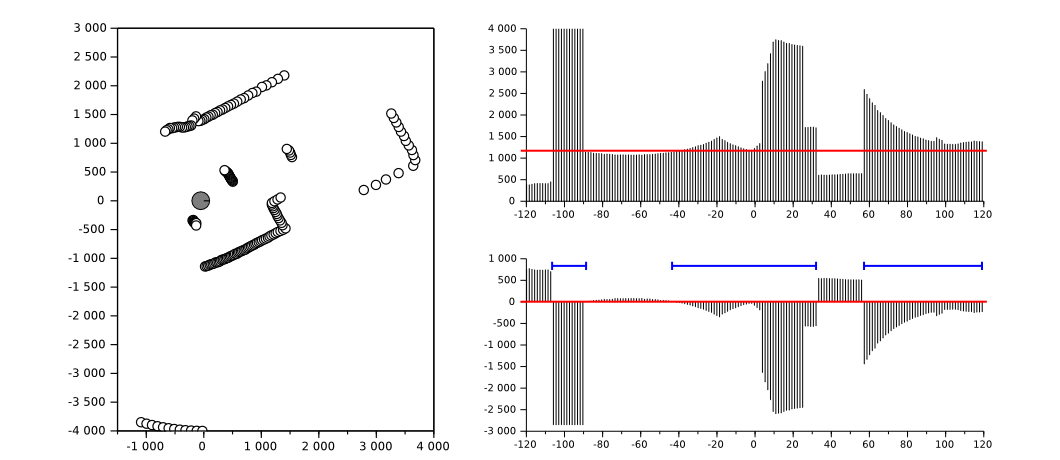
\includegraphics[scale=.37]{figures/VFH.png}
\end{figure}
}

\frame{\frametitle{Vector Field Histogram (VFH)}
A cost function $G$ is then applied to every candidate directions, and the direction which generates the smallest value is then selected:
\begin{equation*}
G = u_{1} \cdot \alpha + u_{2} \cdot \beta + u_{3} \cdot \gamma
\end{equation*}
where
\begin{align*}
	\alpha &= \text{difference between target and candidate direction} \\
	\beta &= \text{difference between current direction and candidate direction} \\
	\gamma &= \text{difference between the previously selected direction and candidate direction}
\end{align*}
$u_{1}$, $u_{2}$ and $u_{3}$ are weighting constants
}

\frame{\frametitle{Vector Field Histogram (VFH)}
\begin{itemize}
	\item Advantages:
	\begin{itemize}
		\item Easily adapt to the data acquired by LiDAR
		\item Efficient Calculation
		\item Adjustable characteristic
	\end{itemize}
	\vspace{0.25cm}
	\item Disadvantages:
	\begin{itemize}
		\item Ignore the kinematic and dynamic constraints
		\item Ignore robot's geometry
		\item \textbf{Direction depends on free-spaces}
	\end{itemize}
\end{itemize}
}

\subsection{Curvature Velocity Method}
\frame{\frametitle{Curvature Velocity Method (CVM)}
CVM takes robot's kinematic constraints into account, assumes it only travels along circular trajectories with curvature $c =  \omega / \nu$,
where $\omega$ is the rotational velocity and $\nu$ is the translational velocity with limits.
\begin{figure}
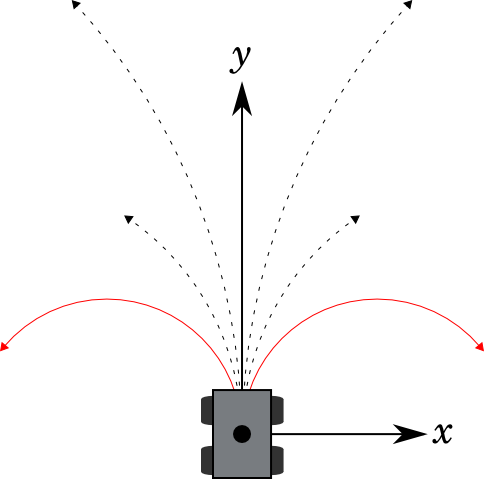
\includegraphics[scale=.35]{figures/CVM1.png}
\end{figure}
}

\frame{\frametitle{Curvature Velocity Method (CVM)}
The travelled distance $d_{v}$ of each obstacle can be calculated, and selected by a cost function.
For real-time implementation, There are some simplifications:
\begin{columns}[t]
\begin{column}{5cm}
	\begin{itemize}
		\item Obstacles are circular shaped
		\item $d_{v}$ between each $c_{min}$ and $c_{max}$ of an obstacle is divided onto few intervals with constant value
	\end{itemize}
\end{column}
\begin{column}{5cm}
	\begin{figure}
	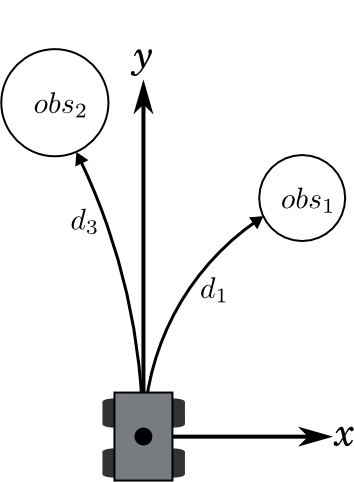
\includegraphics[scale=.35]{figures/CVM2.png}
	\end{figure}
\end{column}
\end{columns}
}

\frame{\frametitle{Curvature Velocity Method (CVM)}
The final decision of new $\omega$ and $\nu$ is made by an object function, which resembles the cost function of previous method:
\begin{equation*}
f(\omega,\nu) = u_{1} \cdot speed(\nu) + u_{2} \cdot dist(\omega,\nu) + u_{3} \cdot head(\omega)
\end{equation*}
where
\begin{align*}
speed(\nu) &= \nu / \nu_{max} \\
dist(\omega,\nu) &= d_{v} / d_{max} \\
head(\omega) &= 1 - |\theta_{target} - \omega \cdot T_{c} | / \pi \\
\end{align*}
The velocities which generate the largest value will be chosen!
}

\frame{\frametitle{Curvature Velocity Method (CVM)}
\begin{itemize}
	\item Advantages:
	\begin{itemize}
		\item Kinematic and dynamic constraints
		\item Robot's geometry constraint
		\item Adjustable characteristic
	\end{itemize}
	\vspace{0.25cm}
	\item Disadvantages:
	\begin{itemize}
		\item Simplified circular obstacle
		\item \textbf{Velocity sensors are required}
	\end{itemize}
\end{itemize}
}

\subsection{Dynamic Window Approaches}
\frame{\frametitle{Dynamic Window Approach (DW)}
DW also assumes the robot only travelled in circular path with rotational velocity $\omega$ and translational velocity $\nu$.
The sensed environment is then transformed into \textbf{velocity space}.
\begin{figure}
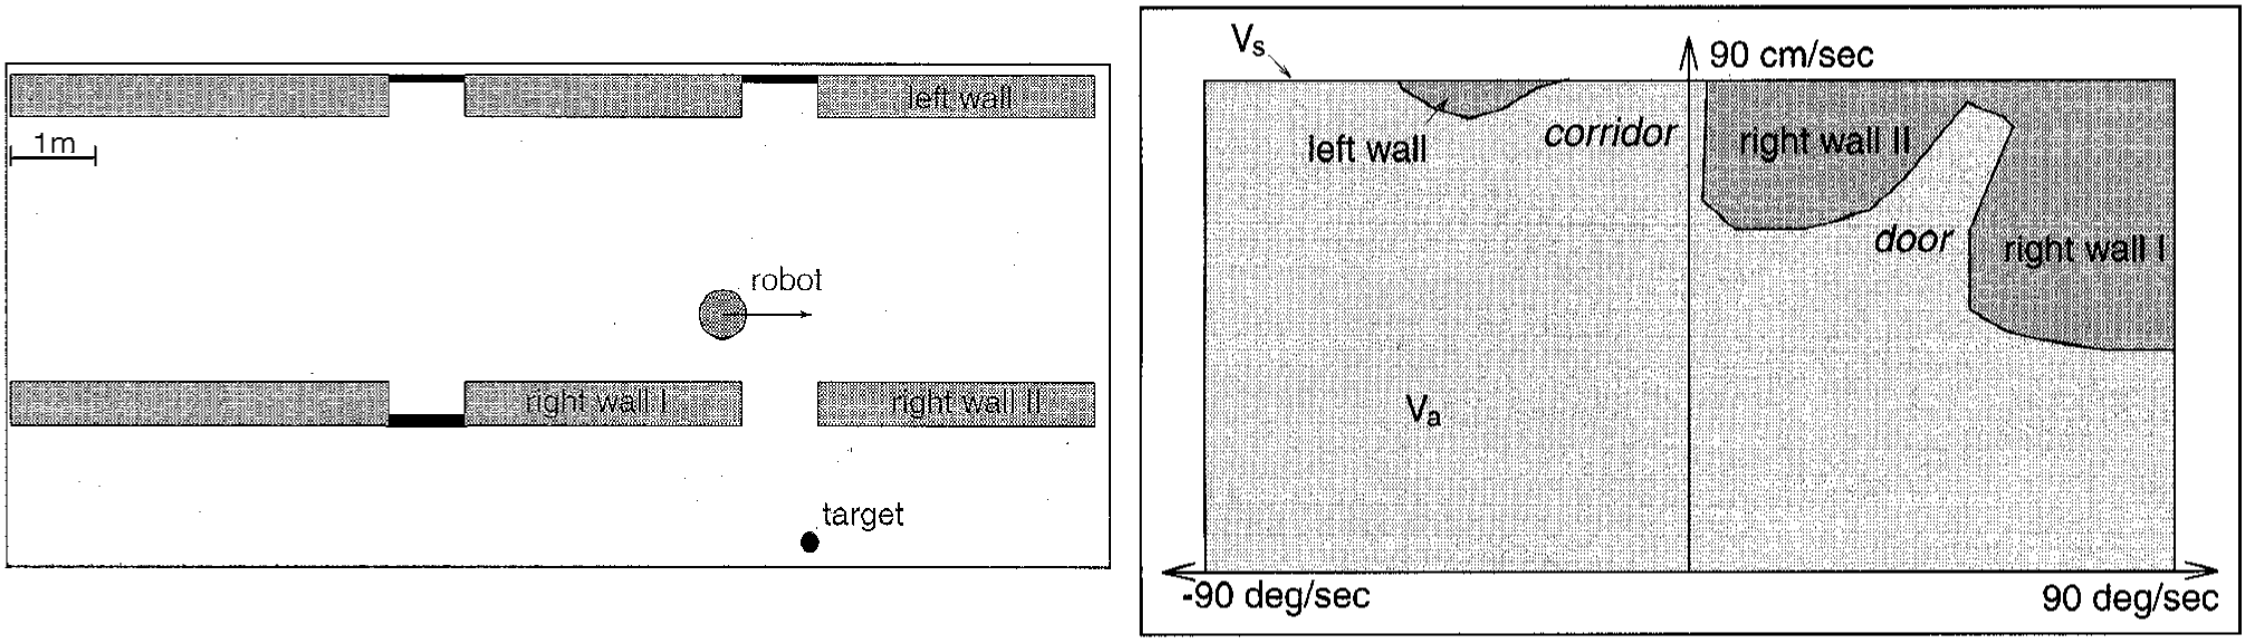
\includegraphics[scale=.17]{figures/DW1.png}
\end{figure}
}

\frame{\frametitle{Dynamic Window Approach (DW)}
In velocity space, a \emph{dynamic window} is constructed according to its dynamic constraints and current velocities.
Again, an object function is used to choose the optimized velocities.
\begin{figure}
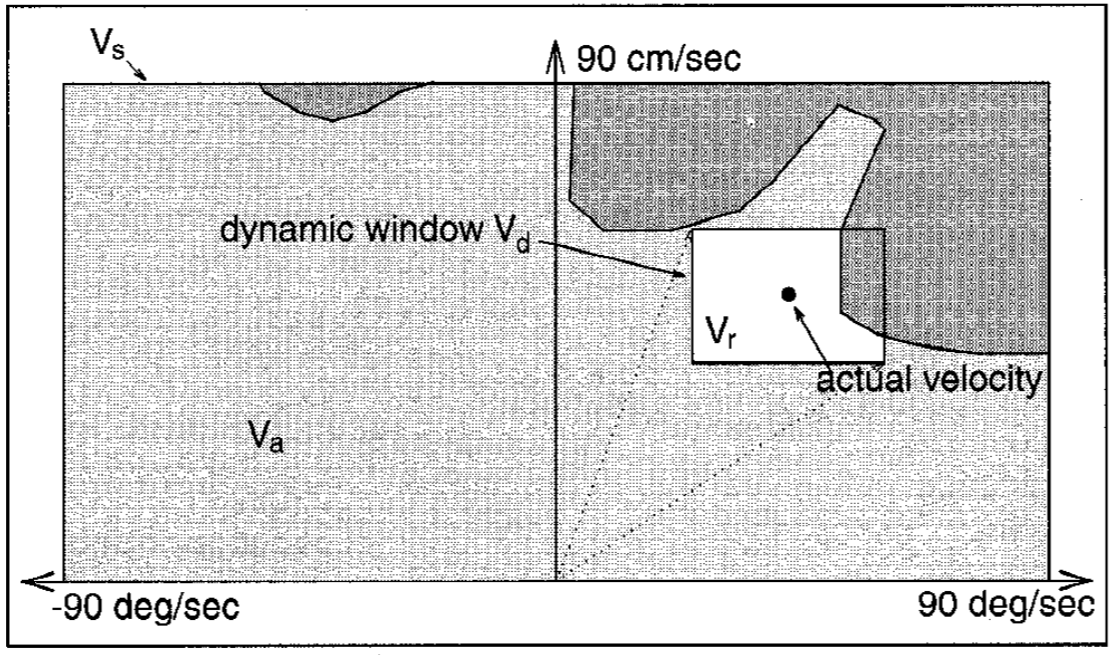
\includegraphics[scale=.25]{figures/DW2.png}
\end{figure}
}

\frame{\frametitle{Dynamic Window Approach (DW)}
\begin{itemize}
	\item Advantages:
	\begin{itemize}
		\item Kinematic and dynamic constraints
		\item Robot's geometry constraint
		\item Adjustable characteristic
	\end{itemize}
	\vspace{0.25cm}
	\item Disadvantages:
	\begin{itemize}
		\item Complexity
		\item \textbf{Velocity sensors are required}
	\end{itemize}
\end{itemize}
}

\section{Vector Field Histogram Plus}
\subsection{Introduction}
\frame{\frametitle{Vector Field Histogram Plus (VFH$^{+}$) - Introduction}
VFH$^{+}$ algorithm is an enhanced version of original VFH which offers several improvements:
\begin{enumerate}
	\vspace{0.25cm}
	\item Kinematic constraints
	\vspace{0.25cm}
	\item Robot's geometry constraints
	\vspace{0.25cm}
	\item \textbf{Direction no longer depends on spaces}
\end{enumerate}
}

\frame{\frametitle{VFH$^{+}$ - Four-Stage Process}
The VFH$^{+}$ employs a four-stage data reduction process in order to compute the new direction of motion:
\begin{enumerate}
	\vspace{0.25cm}
	\item Primary Polar Histogram
	\vspace{0.25cm}
	\item Binary Polar Histogram
	\vspace{0.25cm}
	\item Masked Polar Histogram
	\vspace{0.25cm}
	\item Selection of Steering Direcion
	\vspace{0.25cm}
\end{enumerate}
}

\frame{\frametitle{VFH$^{+}$ - with Laser Range Finder}
However, some modification is required in order to implement VFH$^{+}$ with laser range finder, therefore the process become:
\begin{enumerate}
	\vspace{0.25cm}
	\item Primary Polar Histogram
	\vspace{0.25cm}
	\item Free Spaces
	\vspace{0.25cm}
	\item Blocked Directions
	\vspace{0.25cm}
	\item Selection of Steering Direction
	\vspace{0.25cm}
\end{enumerate}
}

\subsection{Algorithm of Steering Direction}
\frame{\frametitle{1: Primary Polar Histogram}
A polar histogram $P_i$ of corresponding measured distance and angle $d_i$ can be generated with following formula:
\begin{equation*}
	P_i = a + b \cdot d_i
\end{equation*}
\begin{figure}
	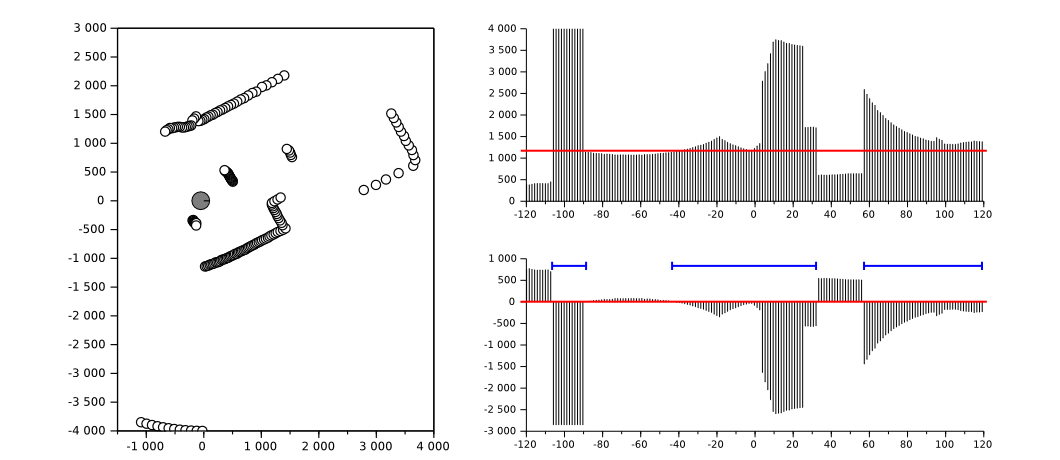
\includegraphics[scale=.33]{figures/VFH.png}
\end{figure}
}

\frame{\frametitle{2: Free Spaces - Hysteresis Filter}
VFH$^+$ uses two thresholds $\tau_{max}$ and $\tau_{min}$ instead of single threshold $\tau$ in VFH
to overcome the oscillation motion in environments with several narrow opennings:
\[
	P'_i = 
	\begin{cases}
		P_i	& \textrm{if } P_i \geq \tau_{max} \\
		0	& \textrm{if } P_i \leq \tau_{min} \\
		P_{i-1}	& \textrm{otherwise}
	\end{cases}
\]
\begin{figure}
	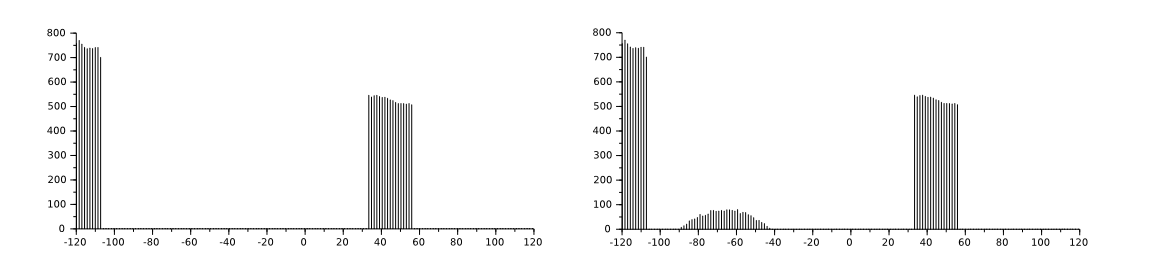
\includegraphics[scale=.35]{figures/HysteresisFilter2.png}
\end{figure}
}

\frame{\frametitle{2: Free Spaces - Boundary}
Each valley of filtered polar histogram $P'_i$ indicates safe directions for the robot, namely $V_j$.
\begin{columns}[c]
	\begin{column}{5cm}
		The boundaries of each $V_j$ are defined by two angle:
		\begin{equation*}
			V_j = (\theta_j^r,\theta_j^l)
		\end{equation*}
	\end{column}
	\begin{column}{5cm}
		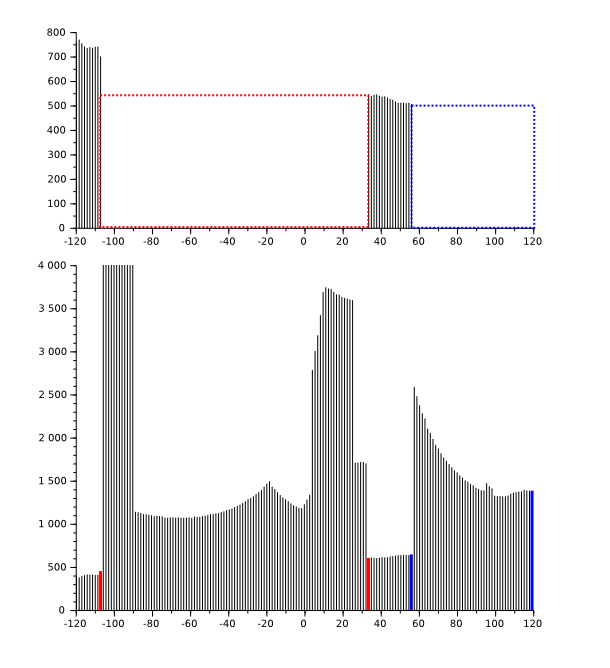
\includegraphics[scale=.32]{figures/FreeSpacesBoundaries.png}
	\end{column}
	
\end{columns}
}

\frame{\frametitle{2: Free Spaces - Robot's Geometry}
With geometry constraints, new boundaries $V_j' = (\theta_j^r{}',\theta_j^l{}')$ of each $V_j$ are calculated:
\begin{columns}[t]
	\begin{column}{5cm}
		\begin{align*}
			\theta_j^r{}'	&= \theta_j^r + \gamma^r \\
					&= \theta_j^r + \arcsin(w_s / d^r)\\
			\intertext{and}
			\theta_j^l{}'	&= \theta_j^l - \gamma^l \\
					&= \theta_j^l - \arcsin(w_s / d^l)\\
			\intertext{where $d^r$ and $d^l$ are corresponding measured distances.}
		\end{align*}
	\end{column}
	\begin{column}{5cm}
		\begin{figure}
		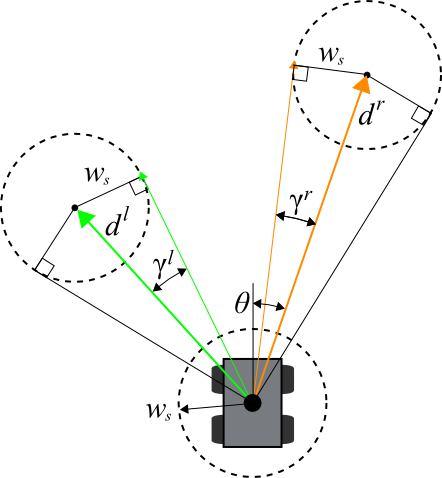
\includegraphics[scale=.4]{figures/Width.png}
		\end{figure}
	\end{column}
\end{columns}
}

\frame{\frametitle{2: Free Spaces - Overlapped}
The $V_j'$ with overlapped boundaries where $\theta_j^r{}' \geq \theta_j^l{}'$ are abandoned, since they are considered too narrow to pass through.
\begin{figure}
	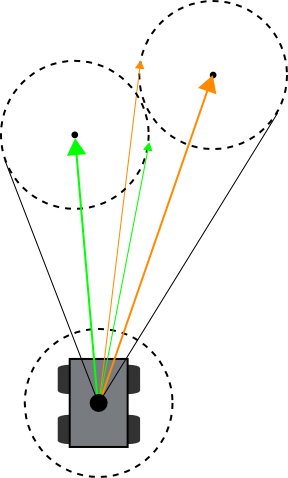
\includegraphics[scale=.4]{figures/WidthOverlapped.png}
\end{figure}
}

\frame{\frametitle{3: Blocked Directions}
VFH$^+$ also assumes circular trajectories of robot's motion.
However, this assumpation only used to determine the limitation of steering angles $\varphi_r$ and $\varphi_l$:
\begin{figure}
	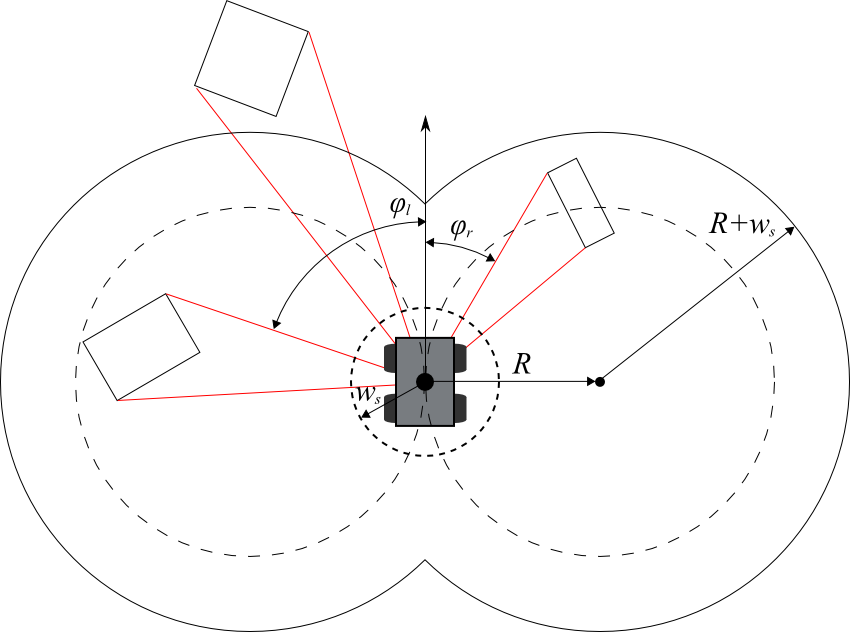
\includegraphics[scale=.3]{figures/Blocked.png}
\end{figure}
}

\frame{\frametitle{3. Blocked Directions - Detection Histogram}
In order to calculate $\varphi_r$ and $\varphi_l$, the detection histogram $D_i$ is generated first:
\begin{equation*}
	D_i = |R\sin\theta_i| + \sqrt{R^2\sin^2\theta_i + w_s^2 + 2Rw_s}
\end{equation*}
\begin{figure}
	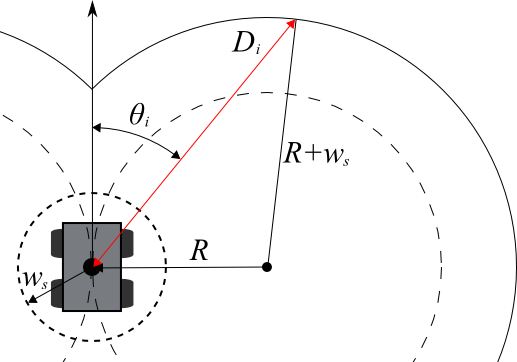
\includegraphics[scale=.4]{figures/DetectionHistogram.png}
\end{figure}
}

\frame{\frametitle{3. Blocked Directions - Masked Histogram}
The masked histogram $M_i = d_i - D_i$ , which shows whethter the steering angle is blocked by obstacles.
\begin{figure}
	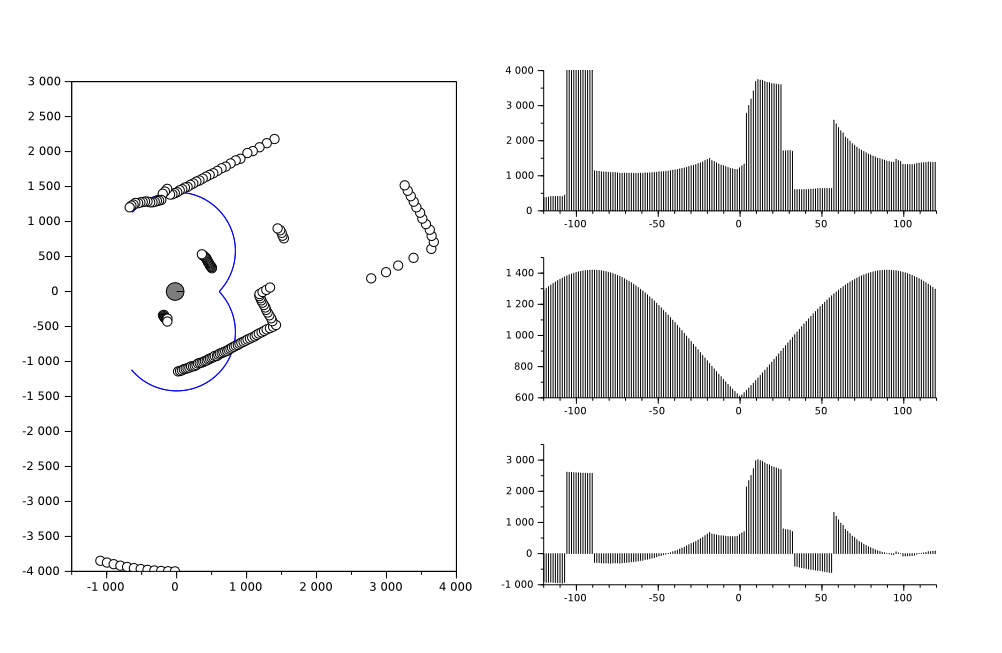
\includegraphics[scale=.35]{figures/MaskedHistogram.png}
\end{figure}
}

\frame{\frametitle{3. Blocked Directions - Determine $\varphi_r$ and $\varphi_l$}
$\varphi_r$ and $\varphi_l$ can be efficiently found by following method: \\
\vspace{0.25cm}
\textrm{1)  Initially set }$\varphi_r = -\pi$\textrm{ and }$\varphi_l = \pi$ \\
\vspace{0.25cm}
\textrm{2) For every }$M_i < 0$\textrm{:} \\
\vspace{0.25cm}
\hspace{0.4cm} \textrm{a) If }$\theta_i < 0$\textrm{ and }$\theta_i > \varphi_r$\textrm{ , set }$\varphi_r$\textrm{ to }$\theta_i$ \\
\vspace{0.25cm}
\hspace{0.4cm} \textrm{a) If }$\theta_i > 0$\textrm{ and }$\theta_i < \varphi_l$\textrm{ , set }$\varphi_l$\textrm{ to }$\theta_i$ \\
}

\frame{\frametitle{4. Selection of Steering Direction - Candidate Direcions}
A set of candidate directions $c_n$ are selected from $\theta_i$ which satisfied:
\[
	\theta_i\in(\varphi_r,\varphi_l) \cap (V_1' \cup V_2' \cup \cdots \cup V_j')
\]
\begin{figure}
	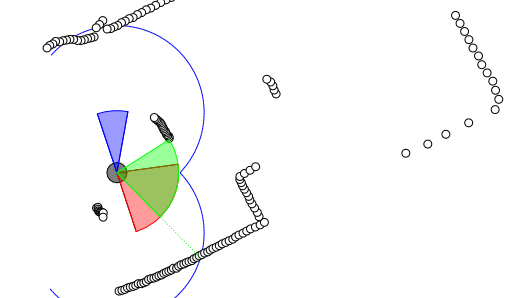
\includegraphics[scale=.5]{figures/CandidateDirections2.png}
\end{figure}
}

\frame{\frametitle{4. Selection of Steering Direction - Cost Function}
Like VFH, VFH$^+$ also uses a cost function to select the preferred direction $c_t$:
\begin{align*}
	G(c_n) &= u_{1} \cdot (|c_n - \varphi_t|) + u_{2} \cdot (c_n) + u_{3} \cdot (|c_n - c_{t-1}|) \\
	\intertext{and}
	c_t &= min \left\{ G(c_n) \right\} \\
	\intertext{where}
	\varphi_t &= \text{Target direction} \\
	c_n &= \text{Candidate direction} \\
	c_{t-1} &= \text{Previously selected directions} \\
\end{align*}
}

\subsection{Algorithm of Speed}
\frame{\frametitle{Algorithm of Speed}
Speed of the robot is controled by the density function $D(d_i)$ of surrounding objects with certain threshold $\tau_{obj}$:
\begin{equation*}
	D(d_i) = \frac{1}{N} \sum_{i=1}^N {H_i}
\end{equation*}
where
\[
	H_i = 
	\begin{cases}
		0	& \textrm{if } d_i \geq \tau_{obj} \\
		1	& \textrm{if } d_i < \tau_{obj} \\
	\end{cases}
\]

With maximum speed $\nu_{max}$ and minimum speed $\nu_{min}$:
\begin{equation*}
	\nu = (\nu_{max} - \nu_{min}) \cdot (1 - D(d_i)) + \nu_{min}
\end{equation*}
}

\subsection{Conclusion}
\frame{\frametitle{Conclusion}
Compare to original VFH method, VFH$^+$ eventually overcomes some defects:
\begin{itemize}
	\item Overcome the primary problem of VFH where steering angle is determined by spaces
	\item Create smooth trajectory by hysteresis threshold
	\item Take robot's geometry and kinematic constraints into account
\end{itemize}
\vspace{0.25cm}
However, it still suffers from some problems:
\begin{itemize}
	\item The geometry of the robot is assumed to be circular
	\item Leads the robot into dead end which can be avoided
\end{itemize}
}

\end{comment}
%\bibliographystyle{abbrv}
%\bibliography{../../thesis/thesis}
\end{document}
